% !TeX program = lualatex
\documentclass[final]{beamer}

\usepackage[size=custom,width=84.1,height=59.4,scale=1.0]{beamerposter}
\usepackage{fontspec}
\usepackage{amsmath,amssymb,mathtools}
\usepackage{graphicx}
\usepackage{xcolor}
\usepackage{tikz}
\usepackage{ragged2e}
\usepackage{booktabs}
\usepackage{enumitem}
\usepackage[most]{tcolorbox}
\usepackage{multicol}
\usepackage{hyperref}
\usepackage[
  backend=biber,
  style=numeric,
  sorting=none,
  giveninits=true,
  maxbibnames=1,
  minbibnames=1,
  url=false,
  doi=false,
  isbn=false,
  eprint=false
]{biblatex}

\addbibresource{refs.bib}
\AtEveryBibitem{%
  \clearfield{eprint}%
  \clearfield{archiveprefix}%
  \clearfield{primaryclass}%
}

\graphicspath{{image/}}

\setmainfont[
  Path = fonts/,
  Extension = .otf,
  UprightFont = *-Regular,
  BoldFont = *-Bold,
  ItalicFont = *-Italic,
  BoldItalicFont = *-Italic
]{HSESans}
\setsansfont[
  Path = fonts/,
  Extension = .otf,
  UprightFont = *-Regular,
  BoldFont = *-Bold,
  ItalicFont = *-Italic,
  BoldItalicFont = *-Italic
]{HSESans}

\definecolor{HSEblue}{cmyk}{1,0.8,0,0.4}
\definecolor{HSElightblue}{cmyk}{0.95,0.75,0,0}
\definecolor{HSEgreen}{cmyk}{0.8,0.1,0.75,0}
\definecolor{HSEred}{cmyk}{0.2,1,0.6,0.05}
\definecolor{HSEorange}{cmyk}{0,0.7,1,0}
\definecolor{HSEink}{HTML}{151A2D}
\definecolor{HSEpaper}{HTML}{FFFFFF}
\definecolor{HSEline}{HTML}{D9E0EE}
\definecolor{HSEsoftblue}{HTML}{EEF4FF}
\definecolor{HSEsoftorange}{HTML}{FFF3EA}

\hypersetup{
  colorlinks=true,
  linkcolor=HSEblue,
  urlcolor=HSEblue,
  citecolor=HSEorange
}

\usetheme{default}
\setbeamertemplate{navigation symbols}{}
\setbeamertemplate{headline}{}
\setbeamercolor{background canvas}{bg=HSEpaper}
\setbeamercolor{normal text}{fg=HSEink}
\setbeamerfont{normal text}{size=\normalsize}
\setbeamersize{text margin left=1.05cm,text margin right=1.05cm}

\setbeamertemplate{footline}{%
  \begin{beamercolorbox}[wd=\paperwidth,ht=0.70cm,dp=0.70cm,center]{poster footer}
    {\color{white}\bfseries\fontsize{11}{13}\selectfont Poster Session \quad|\quad HSE University \quad|\quad GitHub: \texttt{github.com/Oladiy2504/where\_do\_gradient\_methods\_really\_happen}}
  \end{beamercolorbox}
}

\setlength{\paperwidth}{84.1cm}
\setlength{\paperheight}{59.4cm}
\setlength{\parindent}{0pt}
\setlength{\parskip}{0.28em}
\vfuzz=700pt
\hbadness=2000

\newlength{\columnsepwidth}
\newlength{\colwidth}
\newlength{\posterbodyheight}
\setlength{\columnsepwidth}{0.025\textwidth}
\setlength{\colwidth}{0.315\textwidth}
\setlength{\posterbodyheight}{41.6cm}
\setlength{\columnsep}{\columnsepwidth}

\newenvironment{postercol}
  {\begin{column}[T]{\colwidth}\begin{minipage}[t][\posterbodyheight][t]{\linewidth}}
  {\end{minipage}\end{column}}

\newcommand{\posterheader}{%
  \begin{beamercolorbox}[wd=\paperwidth,sep=0cm,leftskip=1.05cm,rightskip=1.05cm]{poster header}
  \vbox to 7.4cm{%
    \vfil
    \begin{columns}[c,totalwidth=\dimexpr\paperwidth-2.1cm\relax]
      \begin{column}{0.16\paperwidth}
        \centering
        
\includegraphics[height=4.75cm,keepaspectratio]{logo.png}
      \end{column}
      \begin{column}{0.68\paperwidth}
        \centering
        {\color{white}\bfseries\fontsize{29}{33}\selectfont\inserttitle\par}
        \vspace{0.34cm}
        {\color{white}\fontsize{15}{18}\selectfont\insertauthor\par}
        \vspace{0.22cm}
        {\color{white}\fontsize{12}{14}\selectfont\insertinstitute\par}
      \end{column}
      \begin{column}{0.12\paperwidth}
        \begin{minipage}[c][5.35cm][s]{\linewidth}
          \raggedleft
          
\includegraphics[height=3.05cm,keepaspectratio]{qr-code.png}\par
          \vfill
          {\color{white}\fontsize{12}{14}\selectfont\insertdate\par}
        \end{minipage}
      \end{column}
    \end{columns}
    \vfil
  }%
  \end{beamercolorbox}
  \nointerlineskip
  \begin{beamercolorbox}[wd=\paperwidth,ht=0.32cm,dp=0cm]{poster stripe}\end{beamercolorbox}
  \vspace{0.6cm}
}

\newenvironment{posterblock}[1]
  {%
    \par\noindent
    {\centering\color{HSEblue}\bfseries\fontsize{22}{25}\selectfont #1\par}
    \vspace{0.16cm}
    {\color{HSEink}\hrule height 0.035cm}
    \vspace{0.26cm}
    \justifying
    \fontsize{16.8}{19.8}\selectfont
  }
  {%
    \par
  }

\newenvironment{highlightblock}[1]
  {%
    \begin{tcolorbox}[
      enhanced,
      width=\linewidth,
      colback=HSEsoftorange,
      colframe=HSEsoftorange,
      boxrule=0pt,
      arc=3mm,
      left=0.48cm,
      right=0.48cm,
      top=0.40cm,
      bottom=0.45cm
    ]
    {\centering\color{HSEblue}\bfseries\fontsize{22}{25}\selectfont #1\par}
    \vspace{0.16cm}
    {\color{HSEink}\hrule height 0.035cm}
    \vspace{0.26cm}
    \color{HSEink}\fontsize{15.4}{18.0}\selectfont\justifying
  }
  {%
    \end{tcolorbox}
  }

\newenvironment{accentblock}
  {%
    \begin{tcolorbox}[
      enhanced,
      width=\linewidth,
      colback=HSEblue,
      colframe=HSEblue,
      boxrule=0pt,
      arc=3mm,
      left=0.42cm,
      right=0.42cm,
      top=0.38cm,
      bottom=0.42cm
    ]
    \color{white}\fontsize{15.0}{17.8}\selectfont\justifying
  }
  {\end{tcolorbox}}

\newenvironment{referencesblock}
  {%
    \par\noindent
    {\centering\color{HSEblue}\bfseries\fontsize{16}{19}\selectfont References\par}
    \vspace{0.12cm}
    {\color{HSEink}\hrule height 0.035cm}
    \vspace{0.16cm}
    \fontsize{6.5}{7.5}\selectfont
    \setlength{\columnsep}{0.45cm}
    \begin{multicols}{2}
  }
  {%
    \end{multicols}
    \par
  }

\newenvironment{widereferencesblock}
  {%
    \par\noindent
    \begin{minipage}{\textwidth}
    {\centering\color{HSEblue}\bfseries\fontsize{17}{19}\selectfont References\par}
    \vspace{0.08cm}
    {\color{HSEink}\hrule height 0.03cm}
    \vspace{0.10cm}
    \fontsize{8.9}{9.7}\selectfont
    \setlength{\columnsep}{0.55cm}
    \begin{multicols}{4}
  }
  {%
    \end{multicols}
    \end{minipage}
    \par
  }

\setbeamercolor{block body}{fg=HSEink,bg=white}
\setbeamercolor{poster header}{fg=white,bg=HSEblue}
\setbeamercolor{poster footer}{fg=white,bg=HSEblue}
\setbeamercolor{poster stripe}{bg=HSEorange}
\setbeamercolor{highlight body}{fg=HSEink,bg=HSEsoftorange}
\setbeamercolor{accent body}{fg=white,bg=HSEblue}
\setbeamertemplate{bibliography item}{\insertbiblabel}
\renewcommand*{\bibfont}{\fontsize{8.9}{9.7}\selectfont}
\setlength\bibitemsep{0.13em}
\setlength{\biblabelsep}{0.2em}   % расстояние между [1] и текстом
\setlength{\bibhang}{1.2em}  

\setlist[itemize]{
  label=\textcolor{HSEorange}{\textbullet},
  leftmargin=1.2em,
  itemsep=0.03em,
  topsep=0.04em
}

\AtBeginDocument{%
  \everymath{\displaystyle}%
}

\makeatletter
\let\HSEposter@fontsize\fontsize
\renewcommand{\fontsize}[2]{%
  \begingroup
  \dimen0=#1pt\relax
  \ifdim\dimen0=24pt\relax
    \endgroup\HSEposter@fontsize{11.2}{13.0}%
  \else
    \endgroup\HSEposter@fontsize{#1}{#2}%
  \fi
}
\makeatother


\title{Where do Gradient Methods Really Happen? Maybe Not Where We Expected}
\author{Artur Babayan\texorpdfstring{\textsuperscript{*}}{*} \and Nikita Musalov\texorpdfstring{\textsuperscript{*}}{*} \and Maksim Kopnev\texorpdfstring{\textsuperscript{*}}{*} \and Aleksey Sivolotskiy\texorpdfstring{\textsuperscript{*}}{*}\and Askar Tsyganov\and Sergey Samsonov}
\institute{HSE University, Moscow, Russia}
\date{\textsuperscript{*}Equal contribution}

\begin{document}

\begin{frame}[t]
\posterheader

\begin{columns}[T,totalwidth=\textwidth]
  \begin{postercol}
    \begin{posterblock}{Intro}
      Modern neural networks are trained in extremely high-dimensional parameter spaces, yet their dynamics often look partly low-dimensional. Recent work observes that gradients may quickly align with a dominant Hessian subspace after only a few training steps.

      The goal of our draft is to separate descriptive geometry from causal optimization mechanisms across architectures, optimizers, and alternative choices of training subspaces.
    \end{posterblock}

    \vspace{2.55cm}

    \begin{posterblock}{Problem}
      Let \(u_t\) be the update produced by an optimizer from the current gradient and optimizer state. For a subspace \(U_t\), we decompose this update into projected and complementary parts:
      \[
        u_t=P_{U_t}u_t+(I-P_{U_t})u_t .
      \]

      We compare three trajectories from the same initialization: full updates, updates restricted to \(U_t\), and updates restricted to the orthogonal complement.

      The central question is causal: does a high-alignment subspace preserve loss decrease and validation quality, or does the complementary bulk component still carry the useful progress?
    \end{posterblock}

    \vspace{2.55cm}

    \begin{posterblock}{Projectors}
      The poster will compare several ways to choose \(U_t\):
      \begin{itemize}
        \item top Hessian eigenspaces, following the dominant-subspace hypothesis;
        \item top Layerwise Momentum subspace  selected by the cumulative energy of singular values
        \item top Adaptive Hessian eigenspace
        \item top Muon (Kronecker) Hessian eigenspace
        \item learnable Projector basis on the Stiefel Manifold
      \end{itemize}
    \end{posterblock}

    \vspace{2.55cm}
    
    \begin{posterblock}{Metrics}
      We measure subspace alignment by
      \[
        \chi_U(v)=\|P_U v\| / \|v\|.
      \]

      Following the reference setup, an exponential moving average of alignment can be used as a switching criterion.

      We also track training loss, update norms, and a projected descent ratio: how much predicted one-step loss decrease remains after projection:
      \[
      \rho_U(v)
      =
      \frac{
      \eta \langle g, P_U v\rangle
      -
      \frac{\eta^2}{2}(P_Uv)^\top H(P_Uv)
      }{
      \eta \langle g, v\rangle
      -
      \frac{\eta^2}{2}v^\top H v
      }.
      \]

      These metrics distinguish geometric overlap from actual optimization and generalization behavior.
    \end{posterblock}

    \vspace{2.55cm}

    \begin{posterblock}{Optimizers}
      We treat the optimizer as part of the geometry, not as a detail outside the projection experiment.
      \begin{itemize}
        \item SGD and SGD with momentum;
        \item Adam and AdamW;
        \item Muon and related matrix-aware updates;
      \end{itemize}
    \end{posterblock}
  \end{postercol}

  \begin{postercol}

    \begin{highlightblock}{Explanation}
      \begin{itemize}
        \item Adaptive Hessian Subspace

          The Adam preconditioner induces a local diagonal metric
\[
P=\operatorname{diag}(\sqrt{\widehat v}+\varepsilon).
\]
We therefore analyze curvature in Adam-whitened coordinates:
\[
\widetilde H=P^{-1/2}HP^{-1/2}.
\]
For top eigenvectors \(Q\), the dominant parameter-space subspace is
\[
S_{\rm adaptive}=P^{-1/2}\operatorname{span}(Q),
\]
and the update is split by the \(P\)-orthogonal projector
\[
\Pi_P=P^{-1/2}QQ^\top P^{1/2},
\qquad
u_{\mathrm{dom}}=\Pi_Pu,\quad
u_{\mathrm{bulk}}=(I-\Pi_P)u .
\]
Thus the dominant and bulk components are orthogonal in the optimizer’s adaptive metric, not necessarily in the Euclidean metric.\\[1.0em]


      \item Muon (Kronecker) Hessian

      The Muon polar update can be represented locally by a two-sided Kronecker preconditioner:
\[
\mathcal M=L\otimes R,\qquad
L=(GG^\top)^{1/2},\quad R=(G^\top G)^{1/2}.
\]
The corresponding whitened Hessian block is
\[
\widetilde H_\ell[D]
=
L^{-1/2}H_\ell[L^{-1/2}DR^{-1/2}]R^{-1/2}.
\]
We extract dominant left/right subspaces \((\widetilde U,\widetilde V)\) by HOOI, yielding the structured subspace
\[
S_{\rm Muon}
=
L^{-1/2}\operatorname{span}(\widetilde U)
\otimes
R^{-1/2}\operatorname{span}(\widetilde V).
\]
The dom component is obtained by projection:
\[
D_{\rm dom}
=
L^{-1/2}\widetilde U\widetilde U^\top
(L^{1/2}DR^{1/2})
\widetilde V\widetilde V^\top R^{-1/2}.
\]
      \end{itemize}
    \end{highlightblock}

    \vspace{1.65cm}

    \begin{highlightblock}{Theoretical results}
\textbf{SGD alignment does not imply projected trainability.}
On a quadratic model
\[
L=\frac12 x^\top\Lambda x+\frac12 y^\top M y,
\qquad
\lambda(\Lambda)\gg\mu(M),
\]
SGD noise amplifies gradient energy in high-curvature directions. In the
isotropic case,
\[
\bar\chi_k
=
\frac{\mathbb E\|P_k\nabla L\|^2}
{\mathbb E\|\nabla L\|^2}
\approx
\frac{k\lambda}{k\lambda+(d-k)\mu},
\]
so the gradient can appear almost fully aligned with the dominant Hessian
subspace when
\[
\lambda/\mu\gg(d-k)/k.
\]

But if we actually train only in that subspace,
\[
\dot\theta=-P_k\nabla L(\theta),
\]
then the bulk variables are frozen:
\[
\dot y=0.
\]
Projected training therefore stops on
\[
\theta^*+U_\perp y
\]
rather than at the true optimum, leaving residual loss whenever \(y\neq 0\).

    \end{highlightblock}


  \end{postercol}

  \begin{postercol}
    \begin{posterblock}{Experiments}
    \centering
  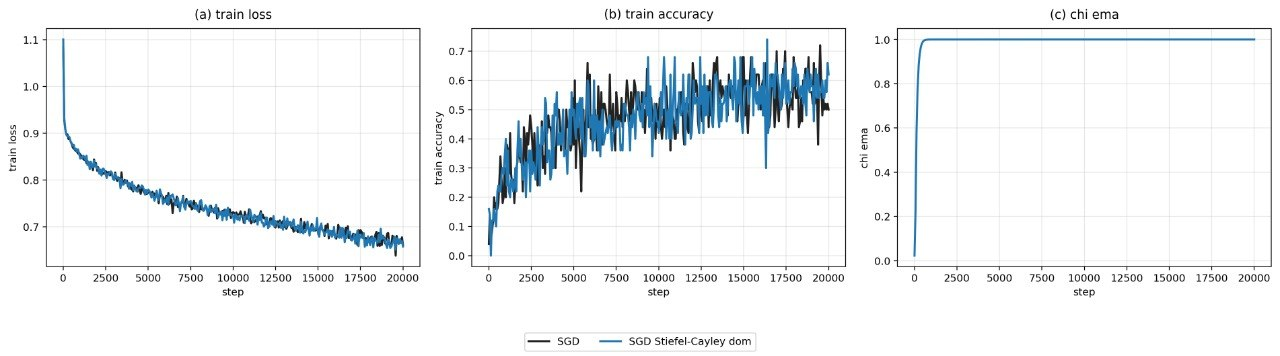
\includegraphics[width=1.0\textwidth]{image/sgd_stiefel_cayley_cnn_cifar.jpg}

  {\fontsize{24}{29}\selectfont
  Projected-training comparison for SGD with a learnable Stiefel projector on CNN on CIFAR10.
  \par}
  \vspace{0.65cm}

    \centering
  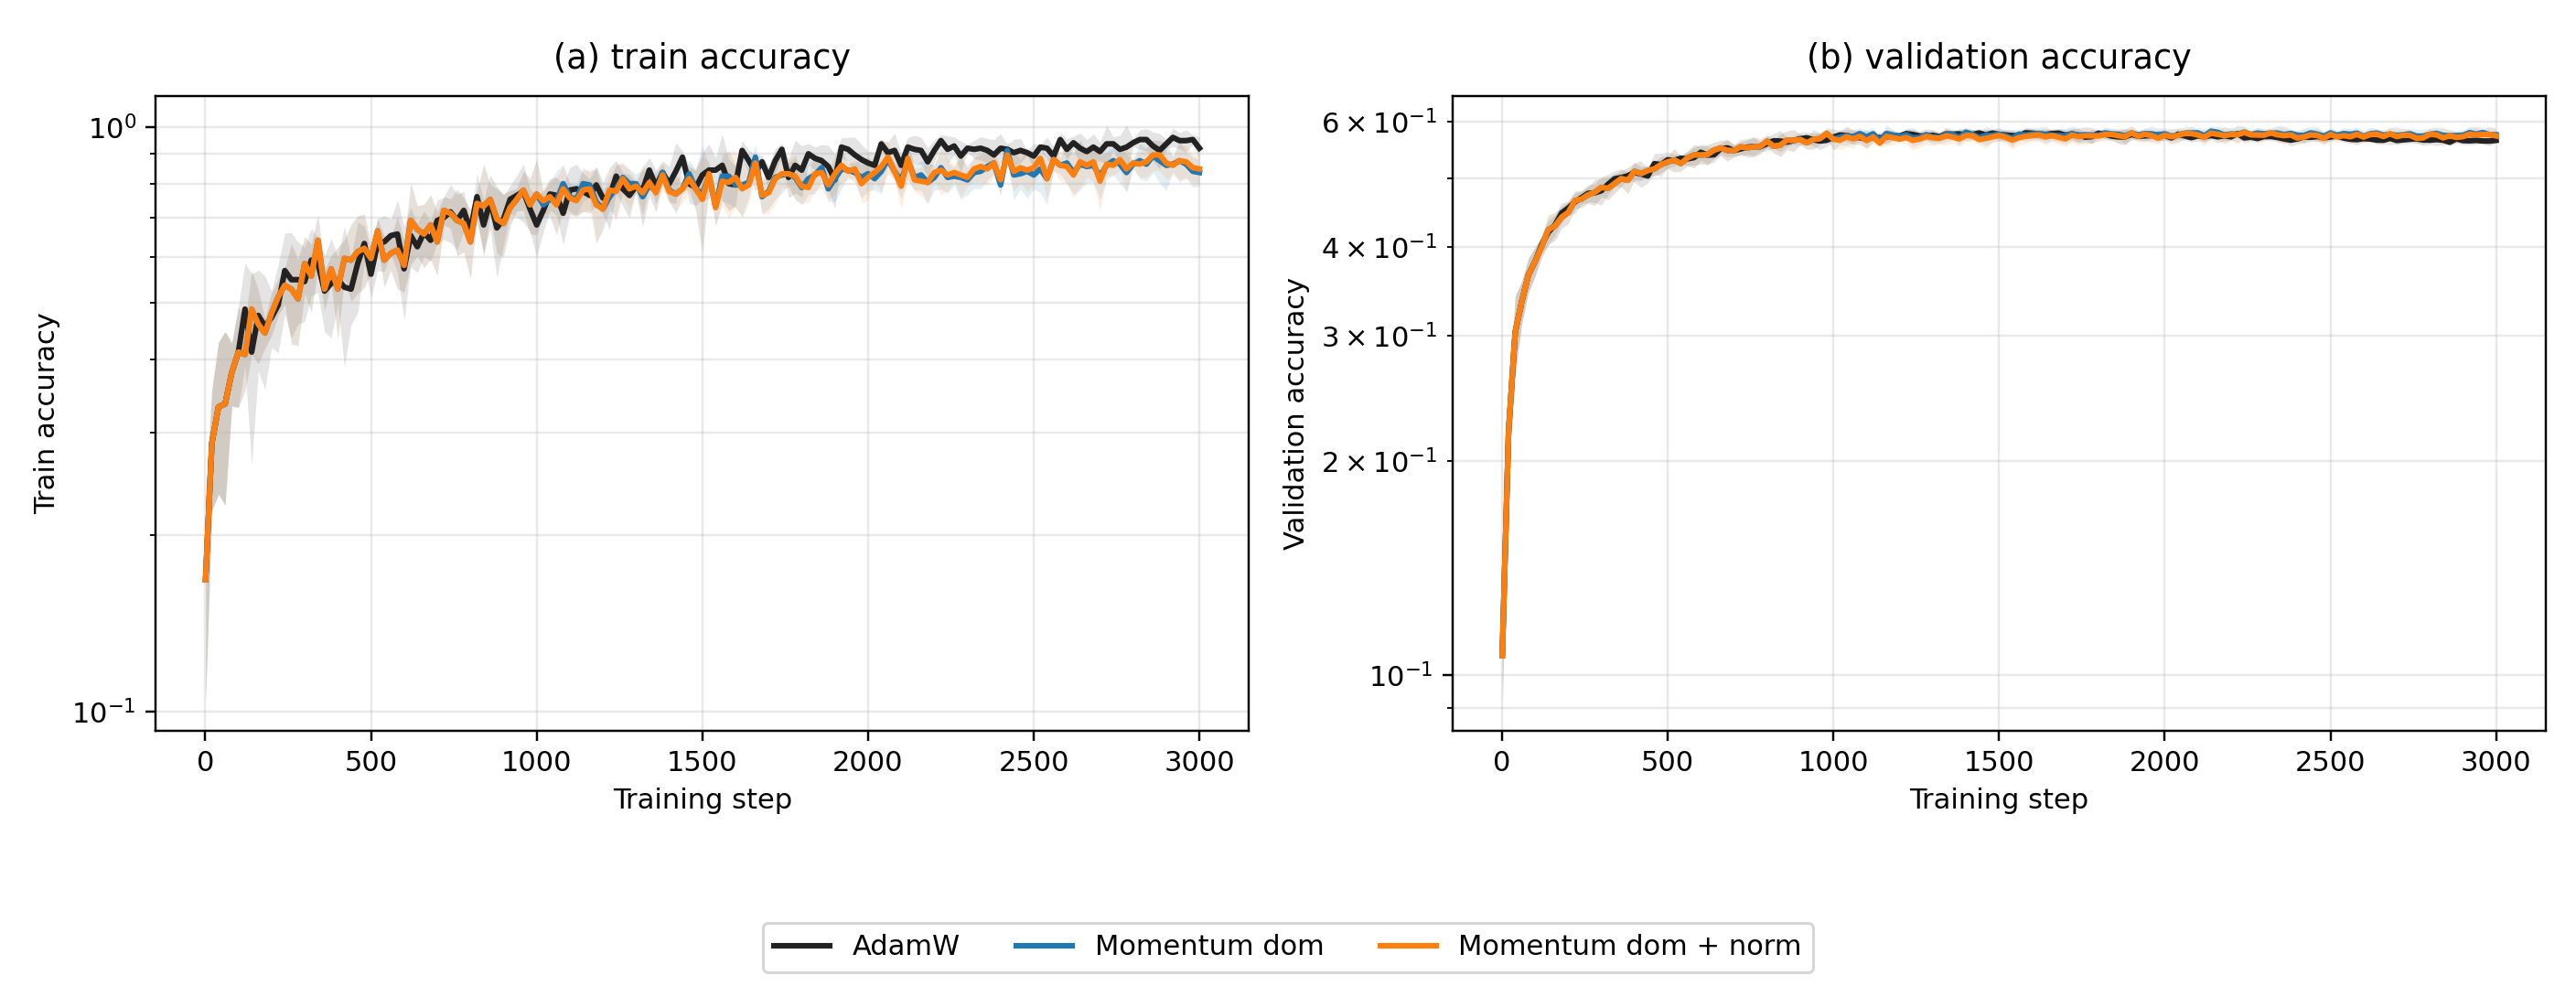
\includegraphics[width=1.0\textwidth]{image/adamw_energy080_norm_correction_accuracy_dashboard.png}

  
  {\fontsize{24}{29}\selectfont
  Projected-training norm correction for AdamW with Layerwise Momentum projector. Norm correction has almost no visible
effect on the behavior of the momentum-induced projection.
  \par}
  \vspace{0.65cm}

    \centering
  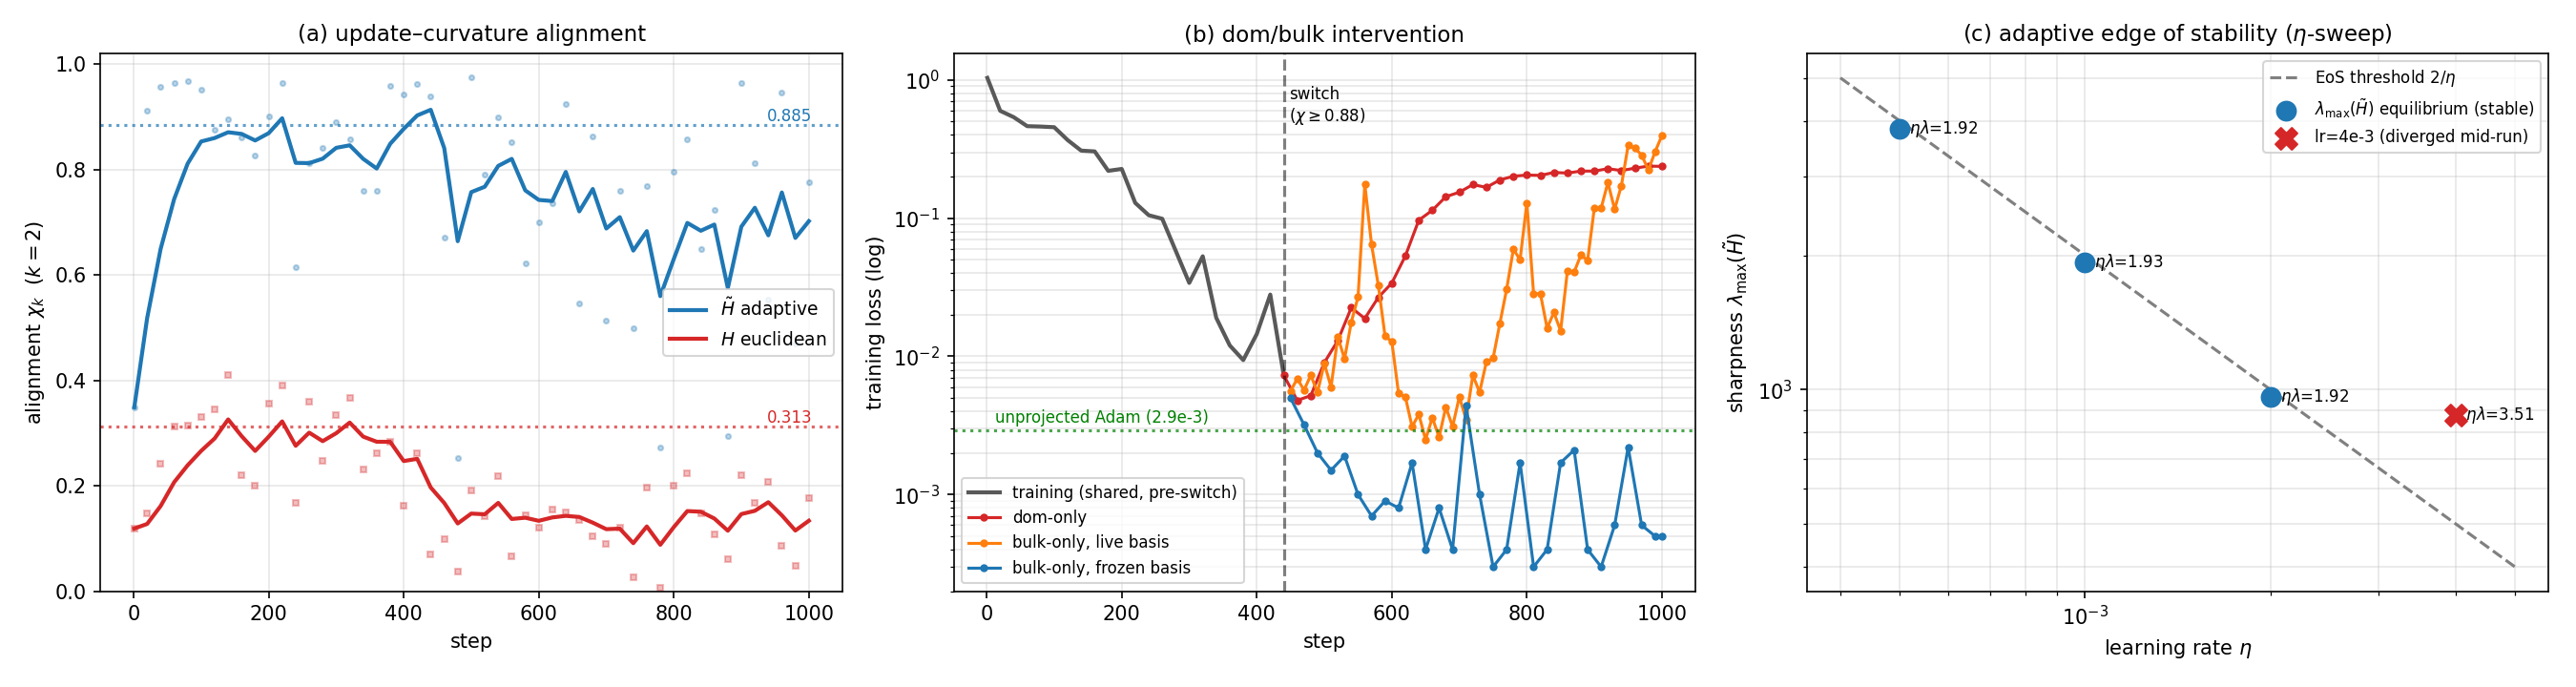
\includegraphics[width=1.0\textwidth]{image/adam_dashboard.png}

  {\fontsize{24}{29}\selectfont
  The update aligns with the top-k subspace of the Adaptive Hessian. Projecting onto that subspace halts training, meanwhile the top eigenvalue of the Adaptive Hessian stays pinned to the EoS threshold.
  \par}
  \vspace{0.65cm}

    \centering
  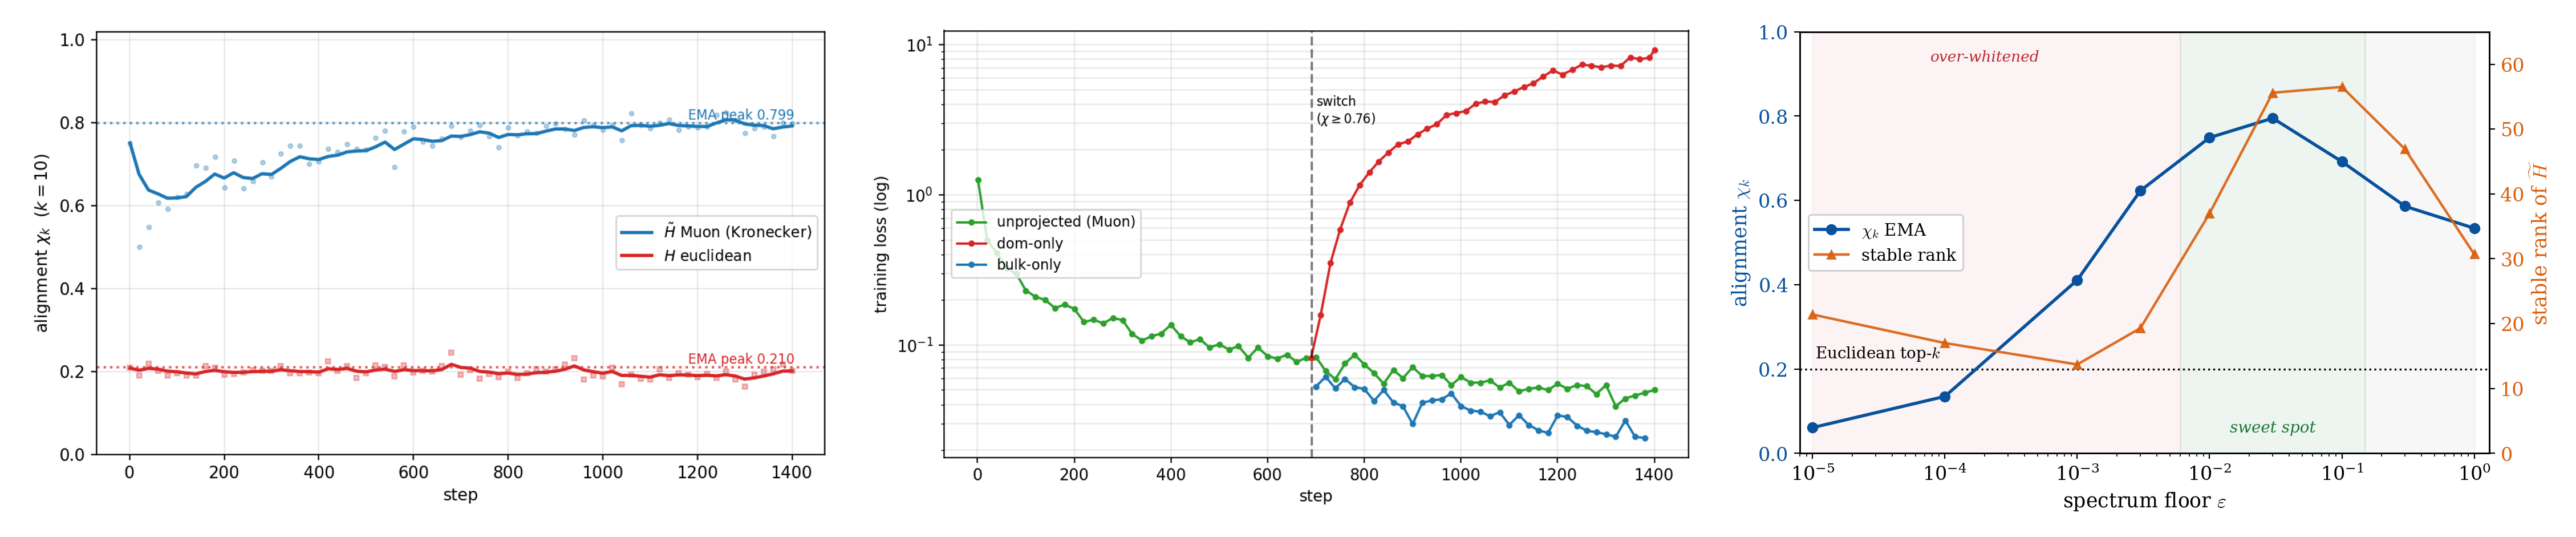
\includegraphics[width=1.0\textwidth]{image/muon_dashboard.png}
  {\fontsize{24}{29}\selectfont
  The update lives in the top-k Muon (Kronecker) Hessian subspace, and projecting onto it makes Muon diverge while the bulk carries the descent below unprojected Muon. The Muon-metric whitening is sharpest at an intermediate spectrum.
  \par}
    \end{posterblock}
    \vspace{0.55cm}

    \begin{accentblock}
      \centering
      \textbf{Acknowledgements}\par
      \vspace{0.18cm}
      This research was supported in part through computational resources of HPC facilities at HSE University, see Kostenetskiy et al.~\cite{hse-hpc}.
    \end{accentblock}
    % \begin{referencesblock}
    %   \nocite{*}
    %   \printbibliography[heading=none]
    % \end{referencesblock}
  \end{postercol}
\end{columns}

\vspace{0.05cm}

\begin{widereferencesblock}
  \nocite{*}
  \printbibliography[heading=none]
\end{widereferencesblock}

\end{frame}

\end{document}
